\subsection{Latencies on Different Weekdays and Diurnal Variation}
\label{sec:latency-weekdays}

It is in question whether TLS handshake latencies vary at different days of the
week. For example, the latency might be different comparing Mondays and
Sundays. To analyze that, we looked at RIPE~Atlas data and Cloudflare~Radar
data.

\subsubsection*{RIPE Atlas}

Using the RIPE Atlas data, we compare different weekdays over the time range of
2022 -- 2024. We were not able to find differences in individual weekdays.
Figure~\ref{fig:latencies-per-weekday} illustrates the latencies that occur in
each weekday as measured by the built-in TLS measurements.

\begin{figure}
	\centering
	\begin{subfigure}[b]{0.32\linewidth}
		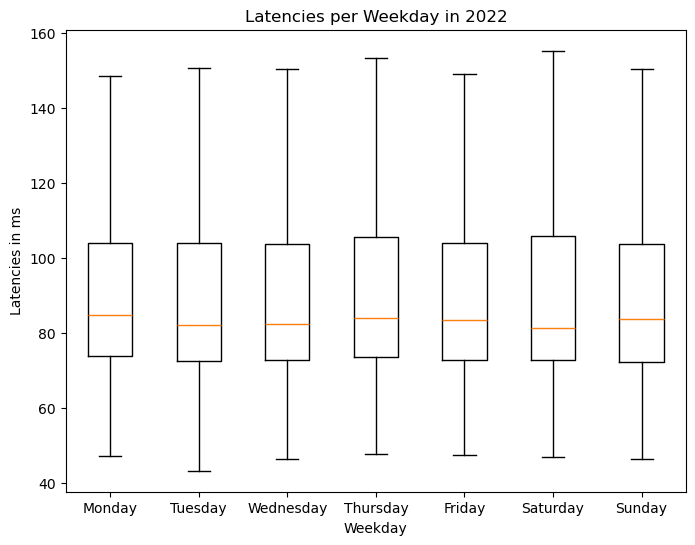
\includegraphics[width=\linewidth]{chapters/4-results/latency/img/latency_2022_weekdays.png}
	\end{subfigure}
	\begin{subfigure}[b]{0.32\linewidth}
		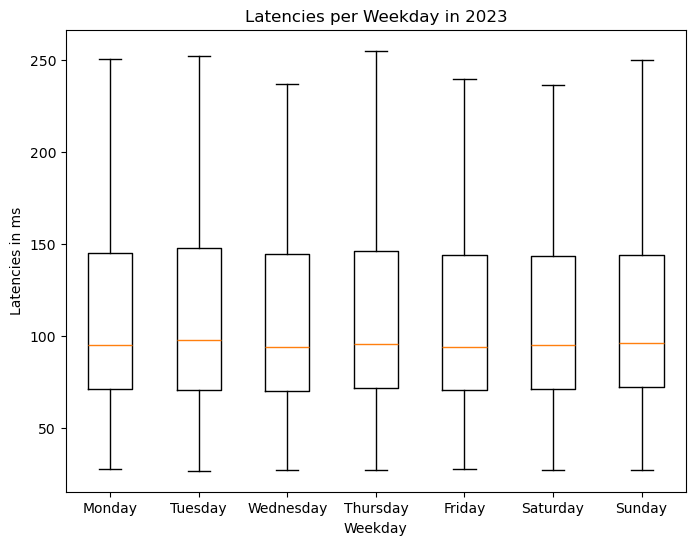
\includegraphics[width=\linewidth]{chapters/4-results/latency/img/latency_2023_weekdays.png}
	\end{subfigure}
	\begin{subfigure}[b]{0.32\linewidth}
		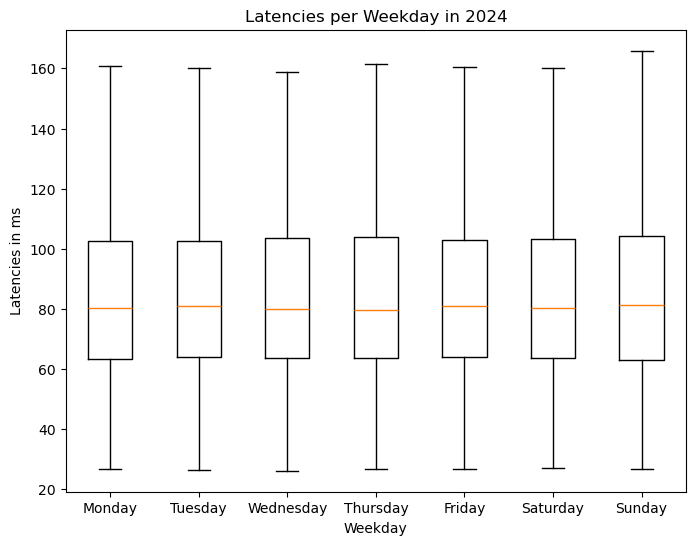
\includegraphics[width=\linewidth]{chapters/4-results/latency/img/latency_2024_weekdays.png}
	\end{subfigure}
	\caption{Latencies from 2022 to 2024 per Weekday.}
	\label{fig:latencies-per-weekday}
\end{figure}

One can see that there is no clear pattern that differentiates the individual
weekdays from the others. This does not change over the course of the years.

To look in more detail on the data, we looked at the data in specific
statistical aggregates (number of measurements, median, average, maximum, and
minimum latency). The results are shown in Table~\ref{fig:weekday-statistics}.

\begin{table}
	\begin{tabular}{llllllll}
		\toprule
		               & Mon. & Tue. & Wed. & Thu. & Fri. & Sat. & Sun. \\
		\midrule
		\textbf{2022}  &      &      &      &      &      &      &      \\
		\#Measurements & 899  & 895  & 904  & 903  & 906  & 918  & 893  \\
		Median         & 84   & 82   & 82   & 84   & 83   & 81   & 83   \\
		Average        & 100  & 100  & 106  & 97   & 99   & 99   & 93   \\
		Maximum        & 1211 & 3090 & 3056 & 703  & 1229 & 1106 & 672  \\
		Minimum        & 47   & 43   & 46   & 47   & 47   & 47   & 46   \\
		\midrule
		\textbf{2023}  &      &      &      &      &      &      &      \\
		\#Measurements & 1448 & 1447 & 1443 & 1429 & 1430 & 1436 & 1462 \\
		Median         & 95   & 98   & 94   & 95   & 94   & 95   & 96   \\
		Average        & 111  & 111  & 108  & 109  & 107  & 108  & 108  \\
		Maximum        & 1245 & 1227 & 1233 & 707  & 1088 & 1220 & 1052 \\
		Minimum        & 28   & 26   & 27   & 27   & 27   & 27   & 27   \\
		\midrule
		\textbf{2024}  &      &      &      &      &      &      &      \\
		\#Measurements & 914  & 930  & 904  & 913  & 914  & 912  & 918  \\
		Median         & 80   & 81   & 80   & 79   & 81   & 80   & 81   \\
		Average        & 97   & 93   & 104  & 105  & 95   & 95   & 95   \\
		Maximum        & 3147 & 1592 & 4374 & 3624 & 4368 & 1230 & 1320 \\
		Minimum        & 26   & 26   & 26   & 26   & 26   & 27   & 26   \\
		\bottomrule
	\end{tabular}
	\caption{Weekday Statistics in Germany}
	\label{fig:weekday-statistics}
\end{table}

They show that the latency does not vary on the individual days. Therefore, you
will not have a worse latency on working days (Monday -- Friday) compared to
the weekend (Saturday and Sunday).

However, the table also allows for an interesting comparison between the years
2022, 2023, and 2024. In 2022, the median TLS handshake latency was between 81
and 84 ms. The average latency was about 20 ms higher. Peak latencies achieved
up to 43 ms. In 2023, the median latencies were significantly higher at 94 to
98 ms. The average latency was in the worst case 14 ms higher, which indicates
a more stable connection, even if the performance was worse compared to 2022.
However, 2023 achieved much better peak performance at 26 ms. In 2024, Starlink
achieved similar median and average latencies compared to 2022, but also
achieving the peak performances from 2023.

\begin{takeaway}{Peak and Average Latency since 2022.}
	Starlink has managed to improve their peak latency by nearly 20 ms
	compared to 2022 while maintaining their median and average latencies.
\end{takeaway}

\subsubsection*{Cloudflare Radar}

Cloudflare offers a different perspective on the data as the data is acquired
differently. We use the Cloudflare Radar data to analyze how Starlink
performance changes over the course of a day. We do that with Cloudflare Radar
data as it offers aggregated data. Similar results are expected for RIPE~Atlas
measurements.

Due to the completeness and availability, we chose to analyze the data from
April 2024. We analyzed individual days as well as the development over the
week. Figure~\ref{fig:latency-per-weekday-1st-2nd-april} shows the latency
development for the first two days in April 2024. It uses the aggregated data
from Cloudflare Radar, which has a resolution of 15 minute intervals.

\begin{figure}
	\centering
	\begin{subfigure}[b]{\textwidth}
		\centering
		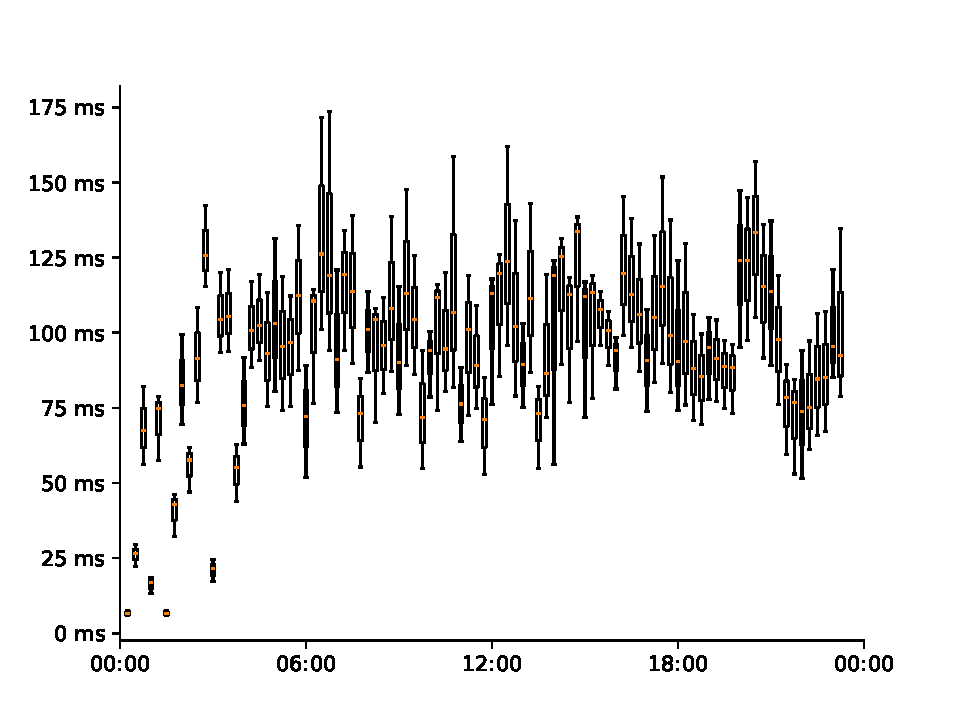
\includegraphics[width=0.8\textwidth]{chapters/4-results/latency/img/cf_radar_latencies_2024-04-01_2024-04-02.pdf}
		\caption{Monday, April 1, 2024 (0:00 -- 24:00)}
	\end{subfigure}
	\begin{subfigure}[b]{\textwidth}
		\centering
		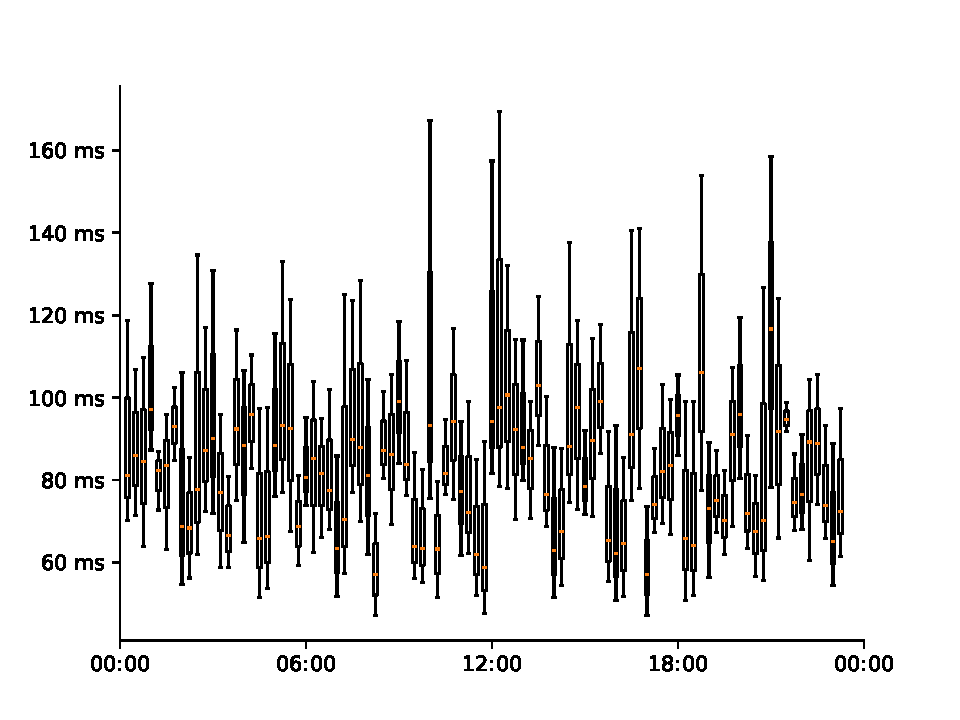
\includegraphics[width=0.8\textwidth]{chapters/4-results/latency/img/cf_radar_latencies_2024-04-02_2024-04-03.pdf}
		\caption{Tuesday, April 2, 2024 (0:00 -- 24:00)}
	\end{subfigure}
	\caption{Cloudflare Radar Latencies of the First Two Days of April 2024}
	\label{fig:latency-per-weekday-1st-2nd-april}
\end{figure}

We expect to observe diurnal variation, as it is also the case for terrestrial
internet connections. While on the first of April, the diurnal variation is
clearly visible, the diurnal variation cannot be clearly seen for the second of
April. However, this day might be an outlier. To further observe diurnal
variation, we observe the rest of the month.
Figures~\ref{fig:latency-per-weekday-weeks-1} and
\ref{fig:latency-per-weekday-weeks-2} show the weeks between April 1 and April
28, 2024.

\begin{figure}
	\centering
	\begin{subfigure}[b]{\textwidth}
		\centering
		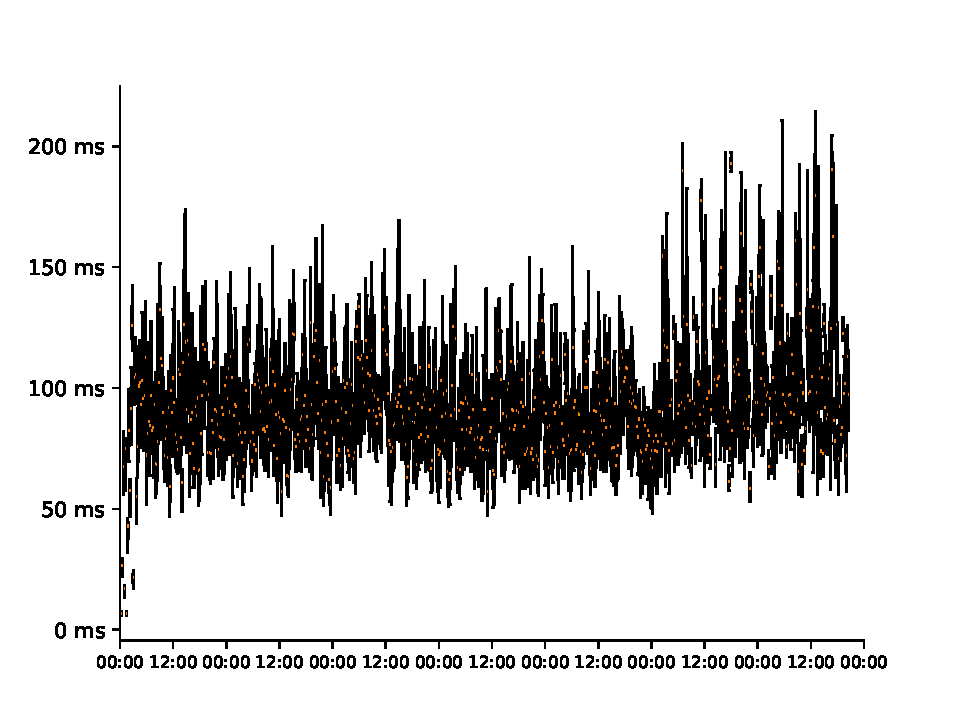
\includegraphics[width=0.8\textwidth]{chapters/4-results/latency/img/cf_radar_latencies_2024-04-01_2024-04-08.pdf}
		\caption{April 1, 2024, to April 8, 2024}
	\end{subfigure}
	\begin{subfigure}[b]{\textwidth}
		\centering
		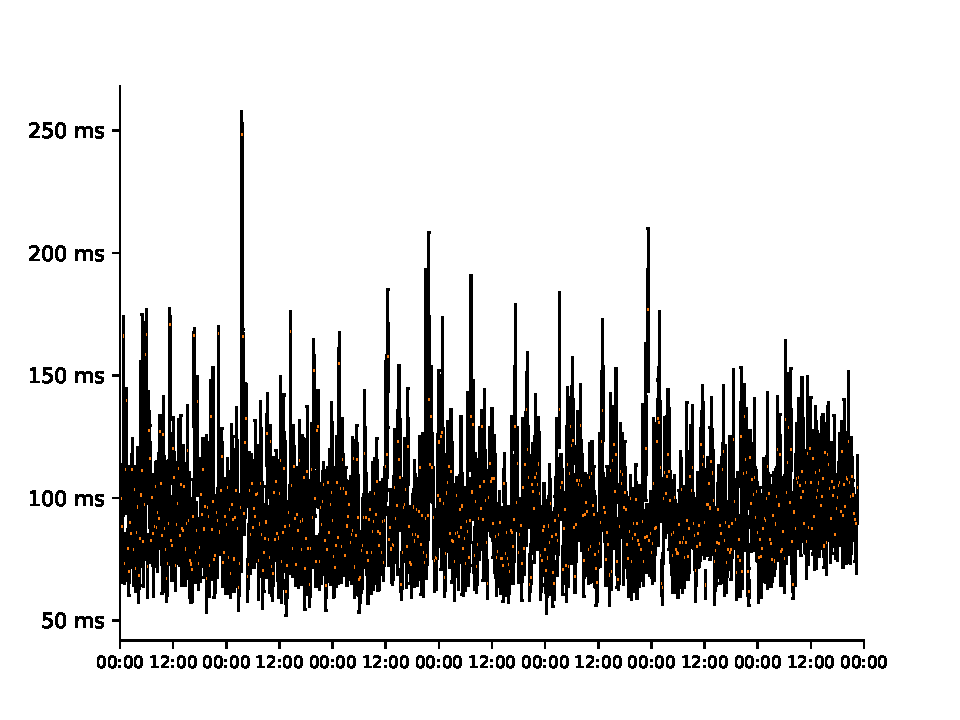
\includegraphics[width=0.8\textwidth]{chapters/4-results/latency/img/cf_radar_latencies_2024-04-08_2024-04-15.pdf}
		\caption{April 8, 2024, to April 15, 2024}
	\end{subfigure}
	\caption{Cloudflare Radar Latencies of the First Two Weeks of April 2024}
	\label{fig:latency-per-weekday-weeks-1}
\end{figure}

\begin{figure}
	\centering
	\begin{subfigure}[b]{\textwidth}
		\centering
		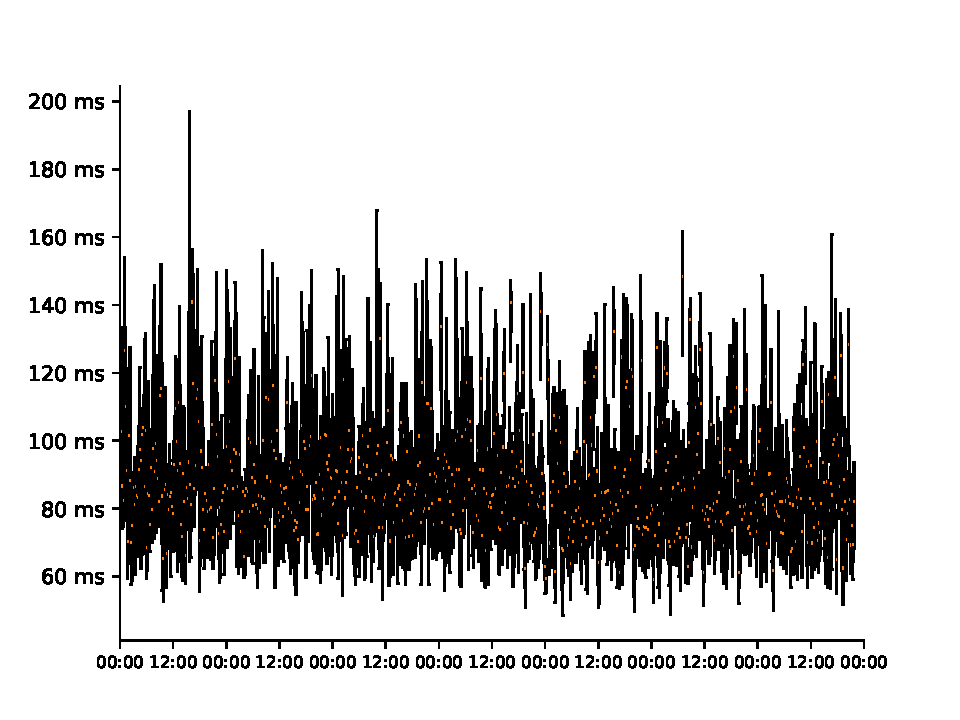
\includegraphics[width=0.8\textwidth]{chapters/4-results/latency/img/cf_radar_latencies_2024-04-15_2024-04-22.pdf}
		\caption{April 15, 2024, to April 22, 2024}
	\end{subfigure}
	\begin{subfigure}[b]{\textwidth}
		\centering
		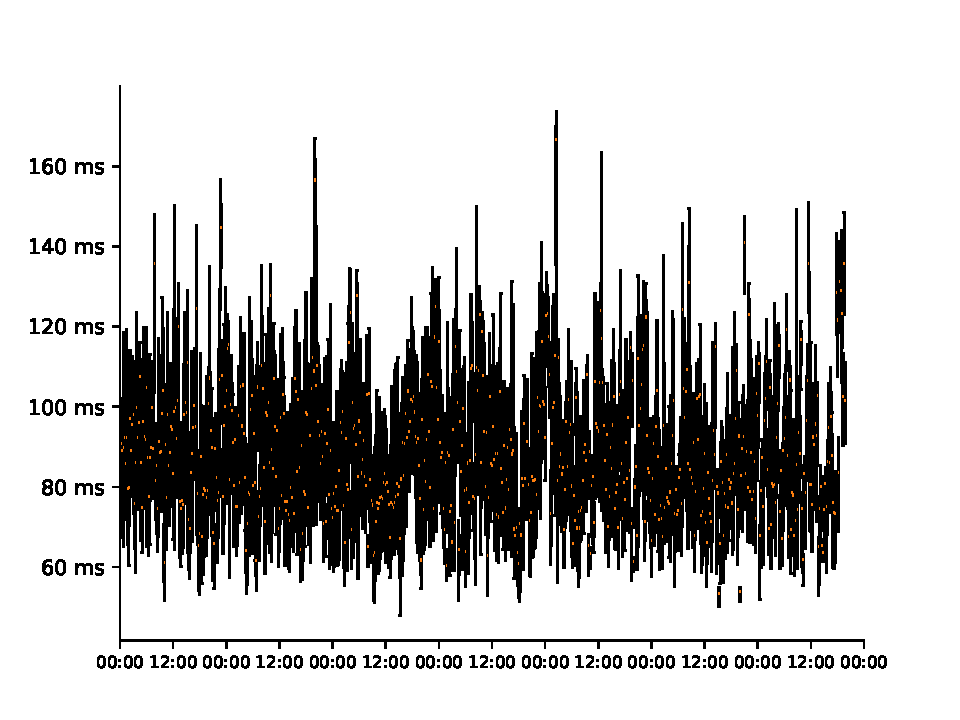
\includegraphics[width=0.8\textwidth]{chapters/4-results/latency/img/cf_radar_latencies_2024-04-22_2024-04-29.pdf}
		\caption{April 22, 2024, to April 29, 2024}
	\end{subfigure}
	\caption{Cloudflare Radar Latencies of the Third and Fourth Week of April 2024}
	\label{fig:latency-per-weekday-weeks-2}
\end{figure}

It is quite clearly visible that in the following weeks there is a strong
variation. This is likely due to diurnal variation. Therefore, we conclude that
Starlink shows a diurnal variation only over the hours of the day, but not
among different weekdays (as shown in Figure~\ref{fig:latencies-per-weekday}
and Table~\ref{fig:weekday-statistics}).

\begin{takeaway}{Diurnal Variation of Starlink}
	Similar to terrestrial internet access, Starlink also shows a clear
	diurnal variation, but only among the hours of the day. The latency
	increases during peak utilization times and is lowest during the night.
	However, there was no observable difference among different weekdays.
\end{takeaway}
